\documentclass[12pt]{article}
\usepackage[utf8]{inputenc}
\usepackage[english]{babel}
\usepackage{amsmath}
\usepackage{amsfonts}
\usepackage{amssymb}

\usepackage[pdftex]{graphicx}
\usepackage{epsfig}
\usepackage{epstopdf}
\usepackage{multirow}

\usepackage{rotating}
%%\usepackage[opciones]{hyperref}



%% MATH -----------------------------------------------------------
\newcommand{\modulo}[1]{\vert#1\vert}
\newcommand{\norm}[1]{\left\Vert#1\right\Vert}
\newcommand{\abs}[1]{\left\vert#1\right\vert}
\newcommand{\set}[1]{\left\{#1\right\}}
\newcommand{\Real}{\mathbb R}
\newcommand{\eps}{\varepsilon}
\newcommand{\To}{\longrightarrow}
\newcommand{\BX}{\mathbf{B}(X)}
\newcommand{\A}{\mathcal{A}}
\newcommand{\Cero}{\mathbf 0}


%% DATOS AUTORES --------------------------------------------------
\author{Pedro Diamel Marrero Fernandez \\ Juan González Hidalgo} 
\title{Projeto AM 2016-1: MVFCMddV e Multiclassificação}

\begin{document}

\maketitle

%\begin{abstract}
%\end{abstract}


\section*{Introdução}
<<<<<<< HEAD

Uma das áreas actualmente mais desenvolvidas do mundo da inteligência artificial é a Aprendizagem de Máquina, na qual se desenvolvem diferentes algoritmos e técnicas que permitem aprender ao computador para seu desenvolvimento em diferentes tarefas.Neste abordagem os algoritmos de agrupamento desempenham um papel fundamental. O objetivo deste trabalho é a implementação e avaliação do método de clusters MVFCMddV( Multi-view relacional fuzzy c-medoids vectors clustering algorithm), assim como a combinação dos classificadores para a classificação de dados utilizando várias funcionalidades(feauters supspaces). Este projeto está organizado da seguinte. Seção \ref{MET} é realizada uma breve descrição dos métodos e algoritmos empregados neste trabalho. Finalmente, os resultados obtidos são avaliados e discutidos na Seção \ref{RD}.

=======
Uma das áreas actualmente mais desenvolvidas do mundo da inteligência artificial é a Aprendizagem de Máquina, na qual se desenvolvem diferentes algoritmos e técnicas que permitem aprender ao computador para seu desenvolvimento em diferentes tarefas. Neste abordagem os algoritmos de agrupamento desempenham um papel fundamental. O objetivo deste projeto é a implementação e avaliação do método de clusters MVFCMddV( Multi-view relacional fuzzy c-medoids vectors clustering algorithm), assim como a combinação dos classificadores para a classificação de dados utilizando várias funcionalidades(feauters supspaces). Este projeto está organizado da seguinte forma: Na seção \ref{MET} é realizada uma breve descrição dos métodos e algoritmos utilizados. Os resultados obtidos são avaliados e discutidos na Seção \ref{RD}.
>>>>>>> 8df3e945e1bd769dcfd7b8a44b6b9b2e2ccc2694

\section{Métodos}\label{MET}

\subsection{Algoritmo MVFCMddV}
<<<<<<< HEAD

MVFCMddV é um algoritmo de agrupamento de vetores c-medoide com uma visão multi-relacional difusa que é capaz de particionar objetos tendo em conta simultaneamente vários matrizes de dissimilaridade. O objetivo é a obtenção de um papel de colaboração dos diferentes matrizes de dissimilaridade, a fim de obter um consenso final de uma partição difusa.
Essas matrizes poderiam ter sido obtidos usando diferentes conjuntos de variáveis e funções de dissimilaridade. Este algoritmo é projetado para dar uma partição difusa e um vetor de medoides para cada cluster difuso assim como aprender a relevância de peso para cada matriz de dissimilaridade por meio da otimização de uma função objetivo. Estes pesos relevantes mudam em cada iteração do algoritmo e são diferentes de um cluster para outro.
=======
MVFCMddV é um algoritmo de agrupamento de vetores c-medoide com uma visão multi-relacional difusa que é capaz de particionar objetos tendo em conta simultaneamente várias matrizes de dissimilaridade.O objetivo é a obtenção de um papel de colaboração das diferentes matrizes de dissimilaridade, a fim de obter um consenso final de uma partição difusa.
Essas matrizes poderiam ter sido obtidas usando diferentes conjuntos de variáveis e funções de dissimilaridade. Este algoritmo é projetado para dar uma partição difusa e um vetor de medoides para cada cluster difuso assim como aprender a relevância de peso para cada matriz de dissimilaridade por meio da otimização de uma função objetivo. Estes pesos relevantes mudam em cada iteração do algoritmo e são diferentes de um cluster para outro.
>>>>>>> 8df3e945e1bd769dcfd7b8a44b6b9b2e2ccc2694


\subsection{Classificador Bayesiano}

O Teorema de Bayes é usado para calcular a probabilidade a posteriori de um evento, dados sua probabilidade a priori e a verossimilhança do novo dado. A descrição anterior é determinada pela seguinte equação:

\begin{equation}
\mathbf{P(w_j\vert x)= \dfrac{p(x\vert w_j) P(w_j)}{p(x)} }
\end{equation}

onde $\mathbf{P(w_j\vert x)}$ é a probabilidade a posteriori, a verossimilhança  é dada pela classe $\mathbf{w_j}$ cujo $\mathbf{p(x\vert w_j)}$ é o maior é mais verossímil de ser a verdadeira classe. E a evidência $\mathbf{p(x)}$ determinada pela equação $\mathbf{\Sigma_{j=1}^{n} p(x\vert w_j) P(w_j)}$ é o fator de escala que garante que a
soma das probabilidades a posteriori é 1.

<<<<<<< HEAD
\subsection{Redes MLP}

Para resolver problemas não linearmente separáveis e de classificação utilizando Redes Neurais Artificias, a alternativa mais utilizada é adicionar uma o mais camadas intermediárias ou escondidas. As redes do tipo perceptron multicamadas $\textbf{(MLP)}$ apresentam uma ou mais camadas intermediárias de neurônios e uma camada de saída. Elas são treinadas com um algoritmo de retropropagação do erro (Back Propagation). O modelo é arranjado em 3 camadas na Figura \ref{fig:mlp}.

=======
\begin{equation}
\mathbf{\hat{p}(x_i\vert w_l)= \dfrac{1}{2\pi^\frac{p}{2}\Sigma_{l}^{\frac{1}{2}}}exp\Bigg[ -\frac{1}{2}(x_i- \hat{\mu_{l}})^{T}\hat{\Sigma}^{-1}(x_i-\hat{\mu_{l}}) \Bigg ]  }
\end{equation}

\begin{equation}
\mathbf{\hat{\mu_{l}}= \dfrac{1}{n_l} \sum_{k=1}^{n_l} x_{lk} }
\end{equation}

\begin{equation}
\mathbf{\hat{\Sigma}= \dfrac{1}{n_l-1} \sum_{k=1}^{n_l} (x_{lk}-\hat{\mu_l}) (x_{lk}-\hat{\mu_l})^T }
\end{equation}

\subsection{Redes MLP}
Para resolver problemas não linearmente separáveis e de classificação utilizando Redes Neurais Artificias, a alternativa mais utilizada é adicionar uma o mais camadas intermediárias ou escondidas. As redes do tipo perceptron multicamadas $\textbf{(MLP)}$ apresentam uma ou mais camadas intermediárias de neurônios e uma camada de saída. Elas são treinadas com um algoritmo de retropropagação do erro(Back Propagation).
O modelo é arranjado em 3 camadas na Figura \ref{fig:mlp}.
>>>>>>> 8df3e945e1bd769dcfd7b8a44b6b9b2e2ccc2694
\begin{figure}[h]
\centering
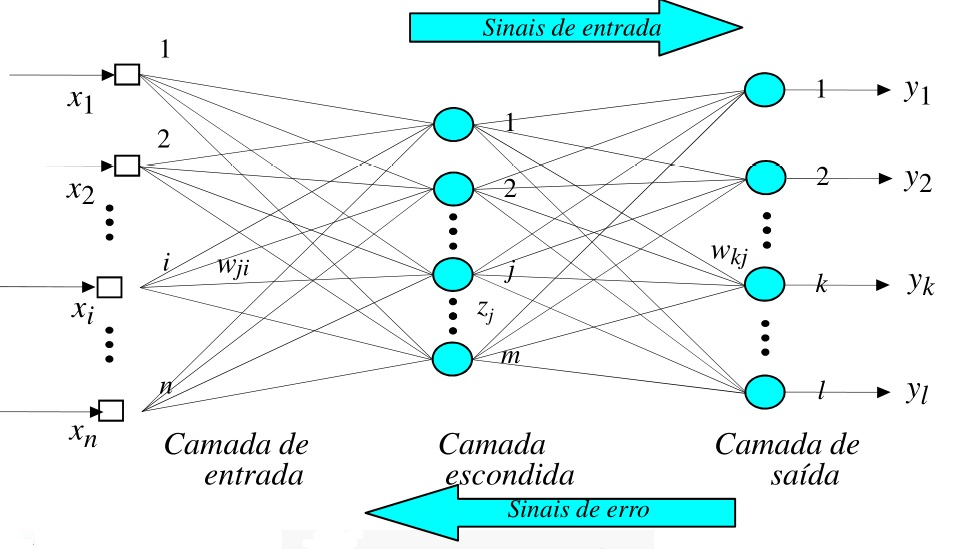
\includegraphics[width=4.5in]{../out/mlp.jpg}
\caption{Rede Neural do tipo MLP}
\label{fig:mlp}
\end{figure} 

Estas redes de tipo $\textbf{MLP-BP}$ tem um alto poder de representação, larga aplicabilidade, facilidade de implementar a aprendizagem e uma boa capacidade de generalização. Mas também seu aprendizagem de transformações complexas pode demorar para convergir, possuem limitações decorrentes do gradiente descendente e a generalização não e garantida(problema de sobretreinamento).

\subsection{Redes SVMs}

As máquinas de vetores de suporte(Support Vector Machines - $\textbf{SVMs}$ ) vêm recebendo crescente atenção da comunidade de Aprendizagem de Máquina nos últimos anos. Elas tem como características principais:
\begin{itemize}
    \item Capacidade de generalização alta, evitando sobretreinamento.
    \item Robustez para categorização de dados com dimensões altas, que tendem a ser sobretreinados em outros classificadores pois muitas micro-características são pouco discriminantes.
    \item Convexidade da função objetivo pois esta é uma função quadrática com apenas um ótimo global. 
    \item Teoria bem estabelecida nas áreas de matemática e estatística.
\end{itemize}

Existem diferentes tipos de redes SVMs, tais como:
\begin{itemize}
    \item SVMs lineares: São usadas na obtenção de fronteiras lineares para a separação de objetos pertencentes a duas classes.
    \item SVMs com Margens Rígidas: Definem fronteiras lineares a partir de dados linearmente separáveis.
    \item  SVMs com Margens Suaves: São definidas para conjuntos que sejam lineramente separáveis.
    \item SVMs não lineares: São eficazes na classificação de conjunto de dados linearmente separáveis ou que possuam uma distribuição aproximadamente linear e a versão de margens suaves tolera a presença de alguns ruídos e outliers.
\end{itemize}

As redes SVMs são comumentes usadas na classificação de padrões, na regressão, no reconhecimento de padrões e no agrupamento. Além disso, elas são desenvolvidas nas áreas de aplicação de detecção de faces em imagens, categorização de textos, regressão linear e bioinformática.



\subsection{Sistema Multi Classificação}


\begin{figure}[h]
\centering
\includegraphics[width=4.5in]{../out/system-multclassy.eps}
\caption{Arquitetura do sistema multiclassificadores utilizada.}
\label{fig:mult_system_classy}
\end{figure}  


\section{Resultados e Discussão}\label{RD}

\subsection{Avaliação do método MVFCMddV em dados sintéticos.}
Para a geração dos dados foi utilizado um gerador aleatorio para dados normais multivariados e três amostras de parâmetros  foram geradas:

$$\mu_1 = [2, 2], \ \mu_2 = [-2, -1], \ \mu_3 = [7, -1] $$
$$\Sigma_1 = \left[ \begin{matrix}
2 & 0 \\ 
0 & 1
\end{matrix} \right], 
\Sigma_2 = \left[ \begin{matrix}
1 & 0 \\ 
0 & 1
\end{matrix} \right], 
\Sigma_2 = \left[ \begin{matrix}
1 & 0 \\ 
2 & 0
\end{matrix} \right] $$

Para gerar três sinais diferentes a partir de uma delas foram rodados os dados em $\theta = 30$ y $\theta = 90$ grados ($X_i = R_i(\theta)*X$). Os resultados obtidos para as três sinais são apresentados na Figura. \ref{fig:xy_sinteticos}.

\begin{figure}[h]
\centering
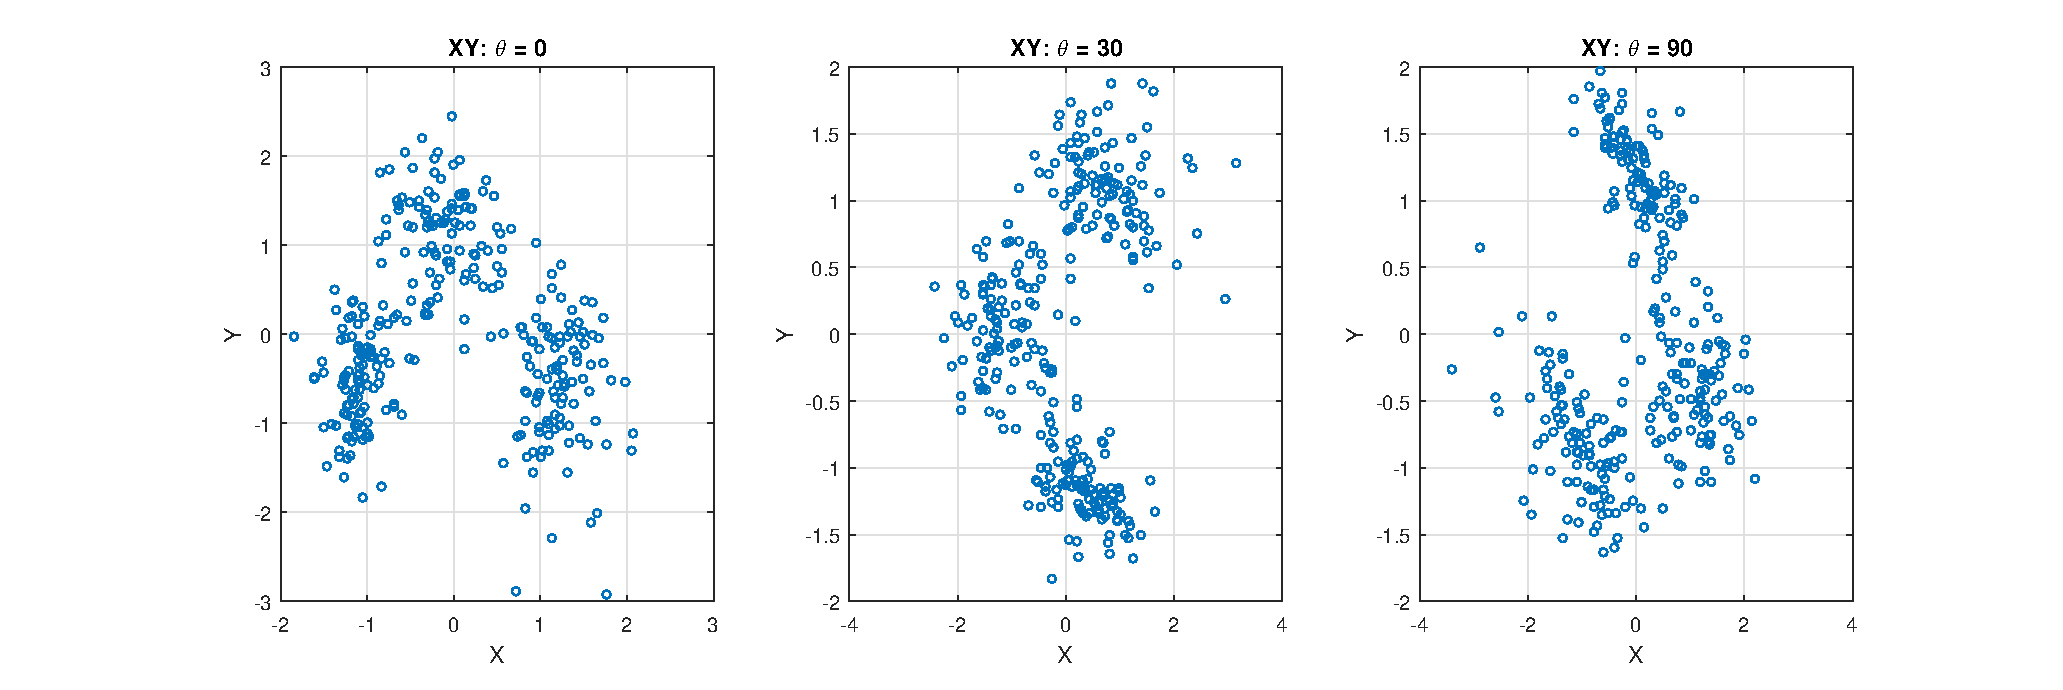
\includegraphics[width=4.5in]{../out/xy-sinteticos.eps}
\caption{Dados sintéticos gerados.}
\label{fig:xy_sinteticos}
\end{figure}  

Para a aplicação do método MVFCMddV foi usada a seguinte configuração, $K = 3$, $m = 1.2$, $T = 10$, $\epsilon = 1e^{-500}$. A Figura \ref{fig:cluster_datos_sinteticos} mostra os resultados obtidos. Neste caso obtive-se um Corrected Rand Index (CR) de $0.98$.

\begin{figure}[h]
\centering
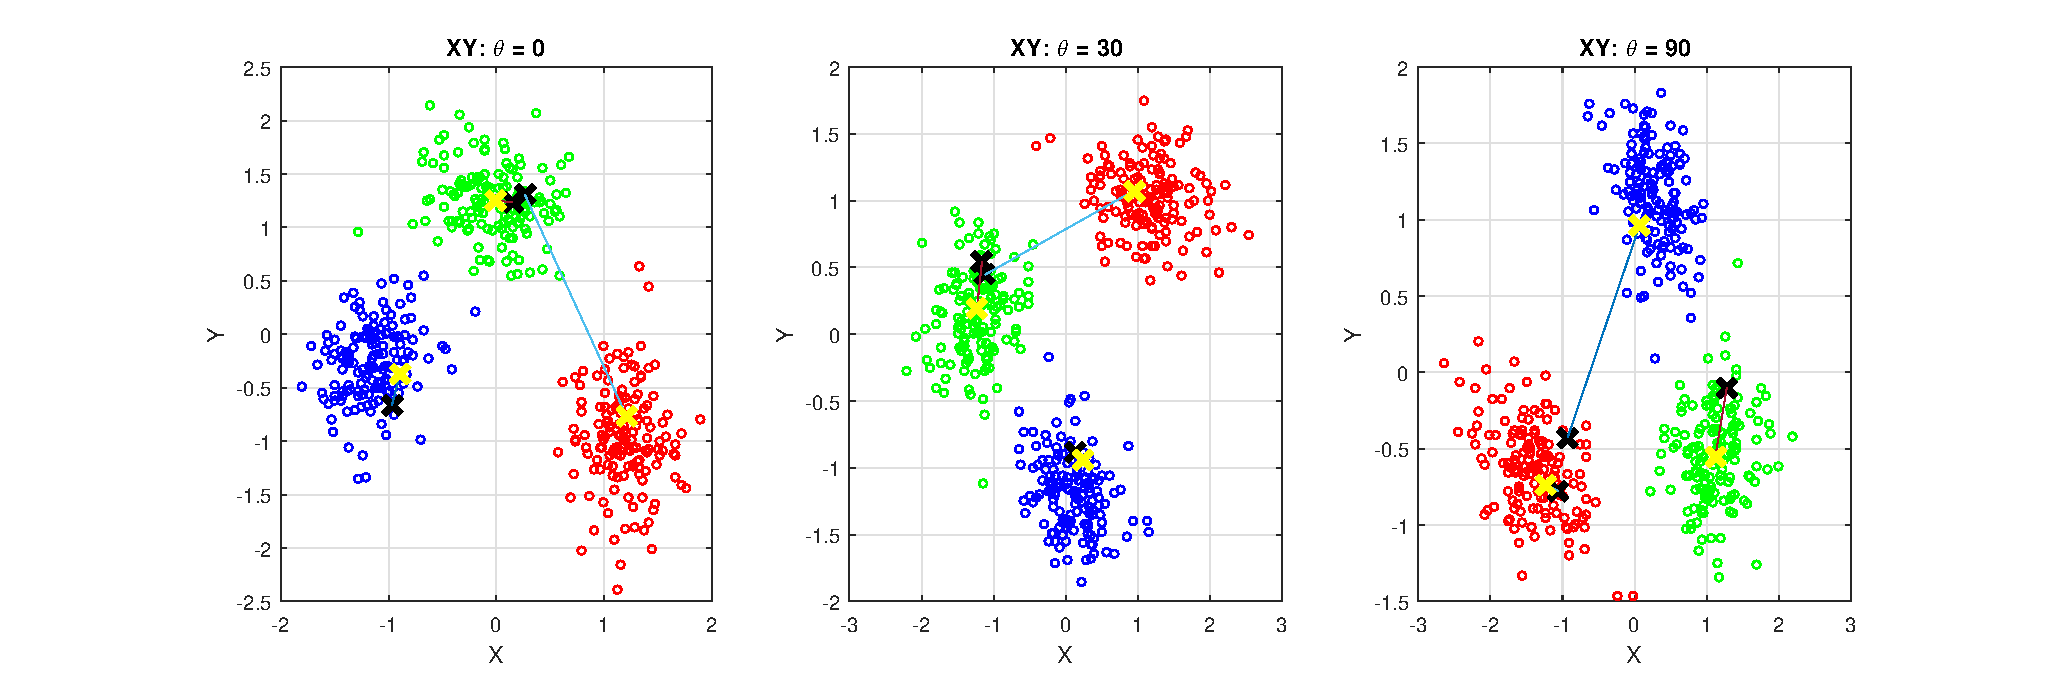
\includegraphics[width=4.5in]{../out/clusters-gauss-3.eps}
\caption{Resultados obtidos pelo MVFCMddV. Os centróides iniciais são mostrados em preto e em amarelo os centróides finais obtidos pelo sistema.}
\label{fig:cluster_datos_sinteticos}
\end{figure}  

\subsection{Avaliação do método MVFCMddV em dados reais.}

Para avaliar o método MVFCMddV com dados reais foi usada Multiple Features Data Set[XXX]. Este conjunto de dados consiste de funcionalidades de números manuscritos (`0'--`9') obtidos a partir de uma coleção de mapas de utilidades holandeses (Figura \ref{fig:data_base}).

\begin{figure}[h]
\centering
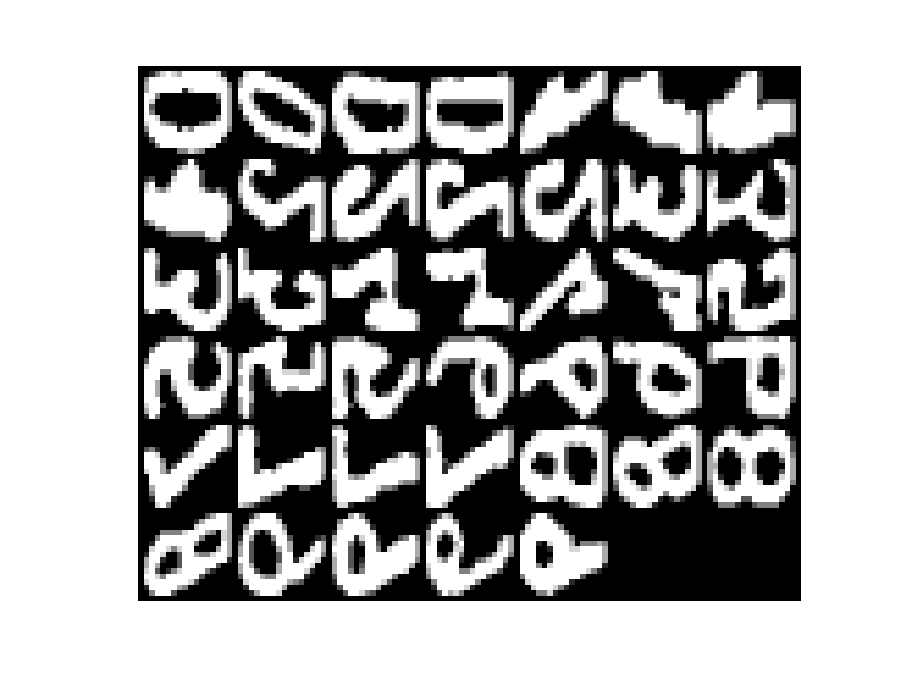
\includegraphics[width=3.5in]{../out/data-base.eps}
\caption{Multiple Features Data Set.}
\label{fig:data_base}
\end{figure}  

<<<<<<< HEAD
Foram digitalizados 200 padrões por classe (para um total de 2.000 padrões) em imagens binárias. Esses dígitos são representados em termos dos seguintes seis conjuntos de características (arquivos):
=======
Foram digitalizados 200 padrões por classe (para um total de 2000 padrões) em imagens binárias. Esses dígitos são representados em termos dos seguintes seis conjuntos de características (arquivos):
>>>>>>> 8df3e945e1bd769dcfd7b8a44b6b9b2e2ccc2694

\begin{enumerate}
\item \textbf{mfeat-fout: (FOUT)} 76 coeficientes de fourier.
\item \textbf{mfeat-fac (FAC):} 216 correlações de perfis.
\item \textbf{mfeat-kar (KAR):} 64 coeficientes Karhunen-Love.
\item \textbf{mfeat-pix (PIX):} 240 médias de pixels em janelas $ 2 \times 3 $.
\item \textbf{mfeat-zer (ZER):} 47 momentos de Zernike.
\item \textbf{mfeat-mor (MOR):} 6 características morfológicas.
\end{enumerate}

<<<<<<< HEAD
Em cada arquivo de 2000 padrões são armazenadas 2000 linhas em ASCII. Os primeiros 200 padrões são de classe`0', seguido por conjuntos de 200 padrões para cada uma das classes `1 '-` 9'. Os padrões correspondentes en diferentes conjuntos de características (arquivos) correspondem ao mesmo caráter original.
A imagem de origem do conjunto de dados é perdida. Usando as versões de amostras  do conjunto de dados PIX das imagems originais podem ser obtidos ($15 \times 16$ pixels).
Para fazer os experimentos foram selecionados os subespaços de características determinados pela FOU, KER e CER. Foi executado 100 vezes ou algoritmo MVFCMddV simultaneamente para as três matrizes de dissimilaridade correspondentes a cada subespaço. Neste caso foi usada a seguinte configuração:$K =10$, $m = 1.6$, $T = 150$, $\epsilon = 1e^{10}$ onde foi obtido um CR index de $0.108$ e um F-mesure de $0.345$. 
=======
Em cada arquivo de 2000 padrões são armazenadas 2000 linhas em ASCII. Os primeiros 200 padrões são de classe`0', seguido por conjuntos de 200 padrões para cada uma das classes `1 '-` 9'. Os padrões correspondentes em diferentes conjuntos de características (arquivos) correspondem ao mesmo caráter original.

A imagem de origem do conjunto de dados é perdida.
Usando as versões de amostras  do conjunto de dados PIX das imagems originais podem ser obtidos ($15 \times 16$ pixels).

Para fazer os experimentos foram selecionados os subespaços de características determinados pela FOU, KER e CER. Foi executado 100 vezes ou algoritmo MVFCMddV simultaneamente para as três matrizes de dissimilaridade correspondentes a cada subespaço. Neste caso foi usada a seguinte configuração: $K =10$, $m = 1.6$, $T = 150$, $\epsilon = 1e^{10}$ onde foi obtido um CR index de $0.108$ e um F-mesure de $0.345$. 
>>>>>>> 8df3e945e1bd769dcfd7b8a44b6b9b2e2ccc2694

\subsection{Método de MVFCMddV em problemas de compactação de imagem.}

Em uma representação de cores de 24 bits de uma imagem simple, cada pixel é representado como três enteiros de 8-bits não assinados (variando de 0 a 255) que especificam o vermelho, verde e azul os valores de intensidade. Esta codificação é muitas vezes referida como a codificação RGB.

Existem outros espaços de representação de cores, tais como CIELAB,HSB CMYK. O objetivo deste experimento é avaliar a redução do número de cores no qual o espaço RGB, utilizando também o espaço CIELAB. Uma hipótese valida é que a informação neste novo espaço pode contribuir para a criação de clusters mais convenientes neste tipo de problemas.

Como pode ser visto na Figura \ref{fig:image_compress} 

\begin{figure}[h]
\centering
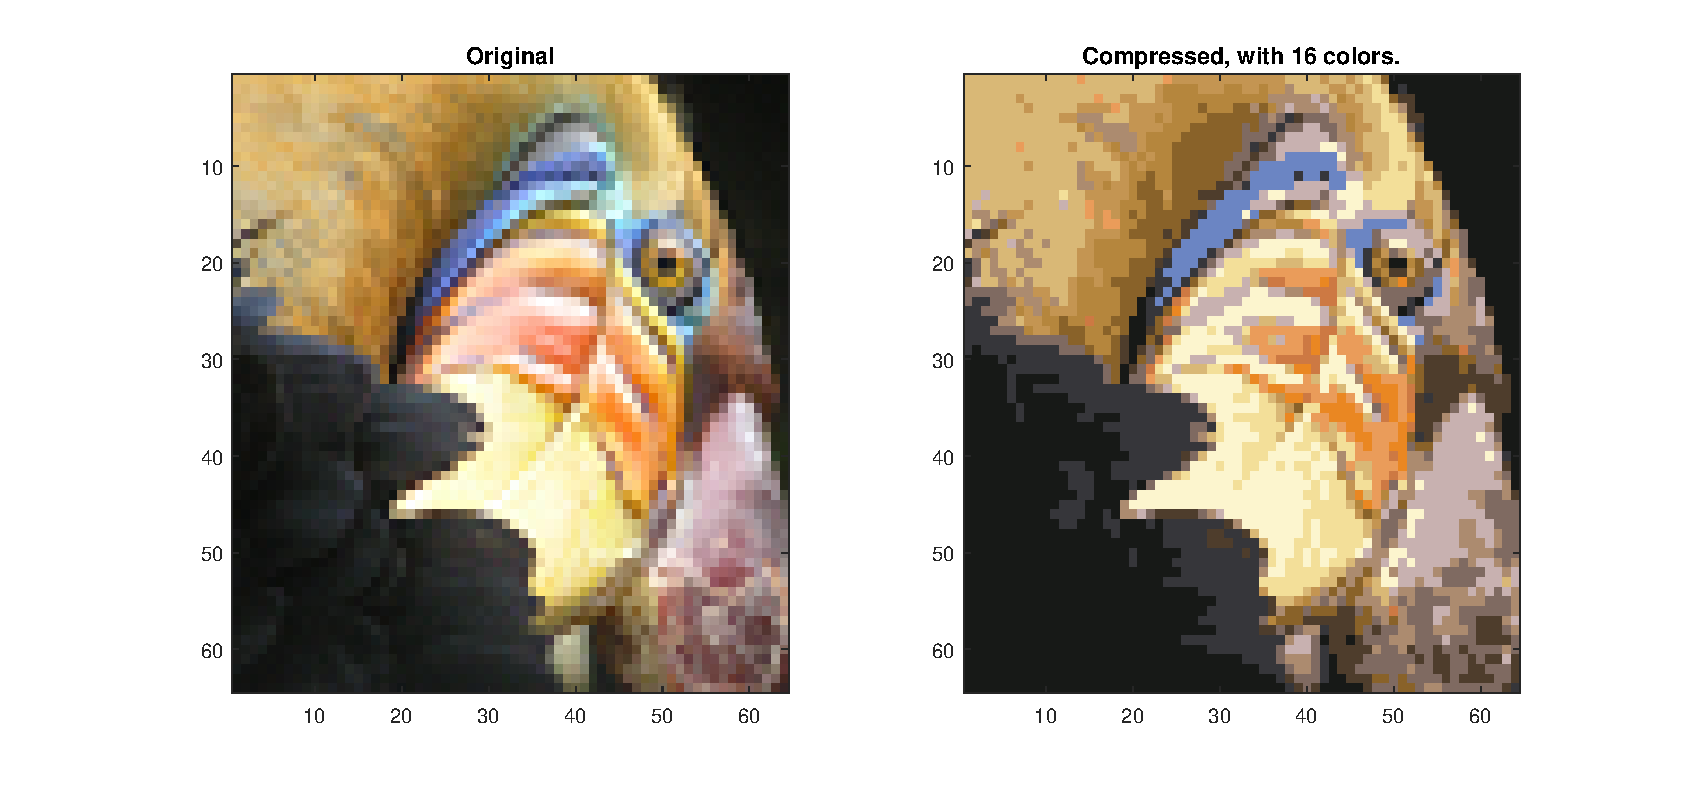
\includegraphics[width=5.5in]{../out/image-compress-16.eps}
\caption{Imagem original e reconstruída (quando se utiliza MVFCMddV para compactar a imagem).}
\label{fig:image_compress}
<<<<<<< HEAD
\end{figure} 
 
uma boa aproximação da imagem original é obtida. Esta nova imagem pode ser apresentada como 4-bits por pixel, mais um dicionário de $16\times24$. A imagem original requer 64 bits para cada um dos $64X64$ das localizações de pixel, resultando em dimensão total de $64\times64\times24 = 98.304$ bits. A nova representação requer alguma sobrecarga de armazenamento na forma de um dicionário de 16 cores, cada uma das quais exigem 24 bits, mas a própia imagem requer só 4 bits por localização de pixel. O número final de bits usado é por conseguinte $16\times24 + 64\times64\times4 = 16.384$ bits, o que corresponde a compressão da imagem original por um factor de aproximadamente 6.
=======
\end{figure}  
uma boa aproximação da imagem original é obtida. Esta nova imagem pode ser apresentada como 4-bits por pixel, mais um dicionário de $16\times24$. A imagem original requer 64 bits para cada um dos $64X64$ das localizações de pixel, resultando em dimensão total de $64\times64\times24 = 98.304$ bits. A nova representação requer alguma sobrecarga de armazenamento na forma de um dicionário de 16 cores, cada uma das quais exigem 24 bits, mas a própia imagem requer só 4 bits por localização de pixel. O número final usado é por conseguinte $16\times24 + 64\times64\times4 = 16.384$ bits, o que corresponde a compressão da imagem original por um factor de aproximadamente 6.
>>>>>>> 8df3e945e1bd769dcfd7b8a44b6b9b2e2ccc2694



\subsection{Sistema multiclasificador para múltiplos sinais}

Neste caso também  foi utilizada a base de dados Multiple Features Data Set. Foi usado o método de validação cruzada com 40 iterações(40-kfold cross validation),  utilizando o conjunto de validação para ajustar os parâmetros dos métodos SVM e MLP. No caso de SVM e MLP  foram ajustados os parâmetros de regularização $C$ e $\lambda$ respectivamente. A Figura \ref{fig:roc_curve} mostra as curvas ROC  que corespondem ao primeiro fold para o ajuste dos parâmetros onde o sinal KAR explica melhor cada uma das classes.


\begin{figure}[!h]
\centering
\begin{tabular}{cc}
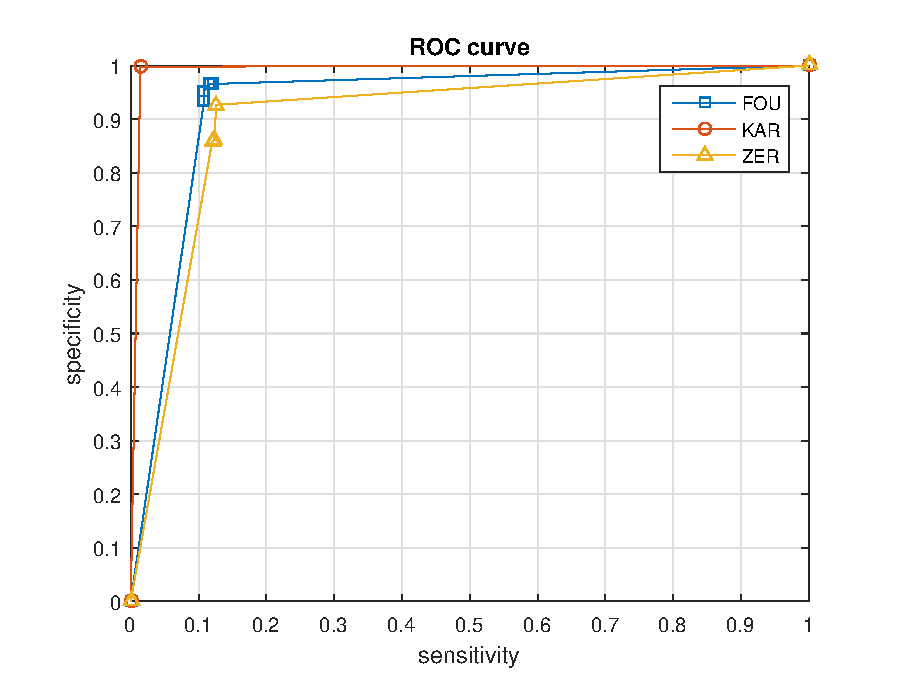
\includegraphics[width=2.5in]{../out/svm-roc.eps}&
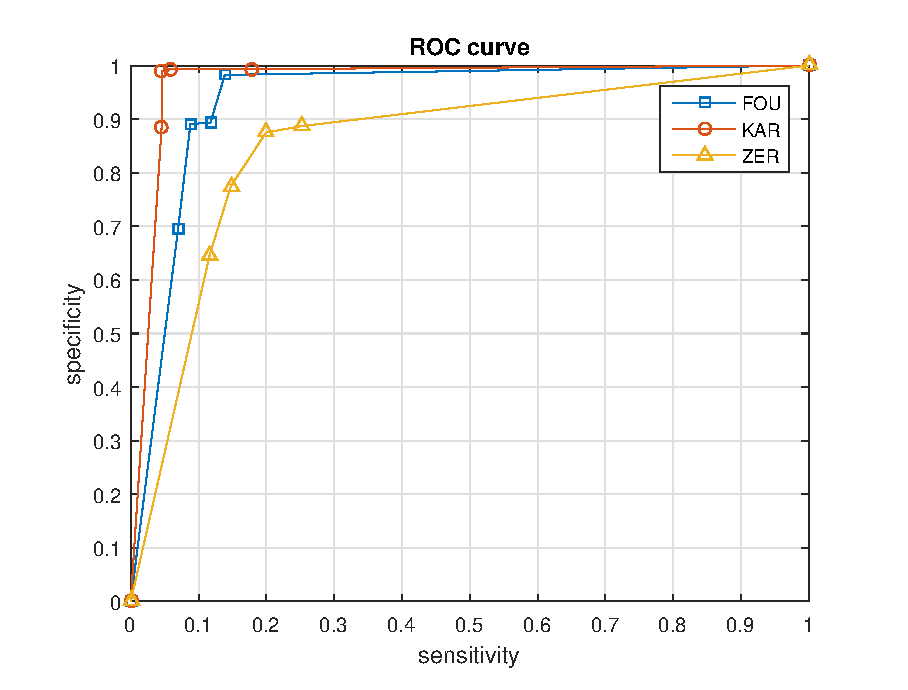
\includegraphics[width=2.5in]{../out/mlp-roc.eps} \\
a) SVM  & b) MLP
\end{tabular}
\caption{Curva ROC variando o termo regularização em cada caso.}
\label{fig:roc_curve}
\end{figure}
 
 
%% Analidis estadistico de los resultados...
%% Analisis de los datos
 
A Tabela \ref{tab:analisis_data} mostra um resumo dos resultados obtidos em cada umo dos algoritmos utilizados de maneira individual contra a combinação de todos (COMB) usando o  voto maioritario (VM). Os melhores resultados foram obtidos utilizando MLP, SVM e COMB com um voto maioritario de $0.92 \pm 0.03$. Todos os métodos foram obtidos para um conjunto de datos de um 0.98 como valor máximo. O abordagem bayesiano teve o pior resultado em uma das iterações.
 
%% R
%%        B              SVM              MLP             ALL        
%% Min.   :0.800   Min.   :0.8600   Min.   :0.860   Min.   :0.8600  
%% 1st Qu.:0.880   1st Qu.:0.9000   1st Qu.:0.895   1st Qu.:0.9000  
%% Median :0.900   Median :0.9200   Median :0.920   Median :0.9200  
%% Mean   :0.901   Mean   :0.9195   Mean   :0.915   Mean   :0.9255  
%% 3rd Qu.:0.920   3rd Qu.:0.9400   3rd Qu.:0.940   3rd Qu.:0.9600  
%% Max.   :0.980   Max.   :0.9800   Max.   :0.980   Max.   :0.9800  
%%> sd(DB$B)
%%[1] 0.037
%%> sd(DB$SVM)
%%[1] 0.035
%%> sd(DB$MLP)
%%[1] 0.032
%%> sd(DB$ALL)
%%[1] 0.034
 
 
\begin{table}[!h]
\renewcommand{\arraystretch}{1.3}
\caption{Resumo dos resultados obtidos.}
\label{tab:analisis_data}
\centering
\begin{tabular}{c}
\begin{tabular}{rcccc}
\hline
         &B   &     SVM  &  MLP   &  COMB     \\
\hline     
 Min.    &0.800   &0.860   &0.860   &0.860\\  
 1st Qu. &0.880   &0.900   &0.895   &0.900\\  
 Median  &0.900   &\textbf{0.920}   &\textbf{0.920}   &\textbf{0.920}\\  
 Sd      &0.037   &0.035   &0.032   &0.034\\
 Mean    &0.901   &0.920   &0.915   &0.926\\  
 3rd Qu. &0.920   &0.940   &0.940   &0.960\\  
 Max.    &0.980   &0.980   &0.980   &0.980\\  
\hline 
\end{tabular}\\
\multicolumn{1}{p{2.8in}}{B: Classificador Bayesiano, SVM: Máquina de Vetor de Suporte, MLP:Perceptron Multi-camadas, COMB: Regra de Combinação pelo Voto Maioritario.}
\end{tabular}
\end{table} 
 
Na Figura \ref{fig:densidade_acc} os resultados são bastante semelhantes na maioria dos casos com uma tendência ao normalidade, principalmente no caso do modelo Bayesiano e MLP. No entanto, a saída do COMB e SVM não parecem ter uma distribuição normal.

\begin{figure}[h]
\centering
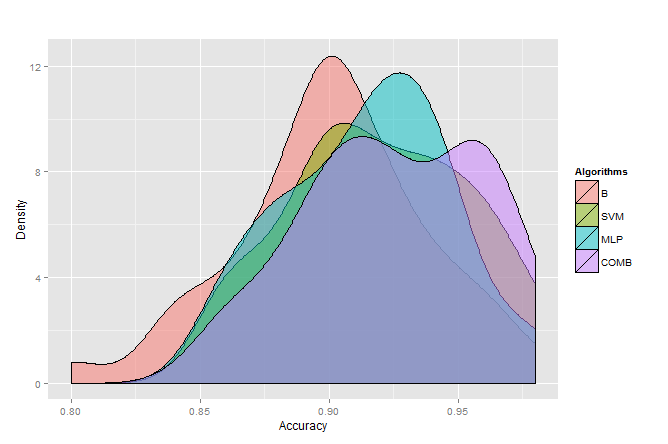
\includegraphics[width=4.5in]{../out/density-graph.png} \\
\caption{Grafico de densidade das amostras correspondentes à saída do erro de cada método testado.}
\label{fig:densidade_acc}
\end{figure} 

A Figura \ref{fig:boxplot_acc} indica que o método COMB não é simétrico, por isso este método tem um maior volume de informações entre o segundo e o terceiro quartil. Este gráfico também nos permite perceber que o comportamento dos métodos é muito semelhante. No caso do modelo Bayesiano apresenta um outliner, indicando que em pelo menos uma iteração do kfold teve resultados debaixo de 0.85.

\begin{figure}[!h]
\centering
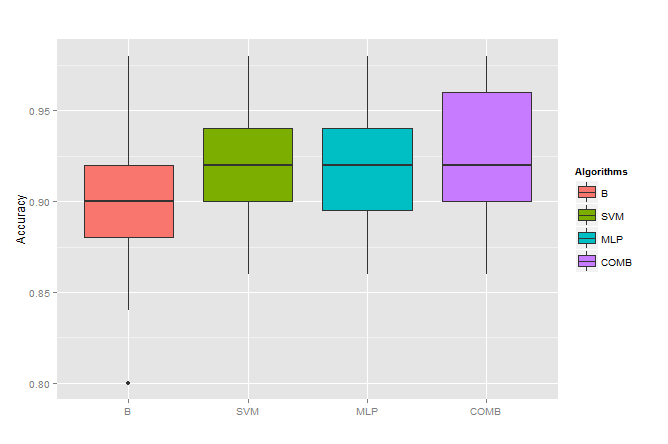
\includegraphics[width=4.5in]{../out/boxplot-errors.png}
\caption{Box plot dos métodos avaliados.}
\label{fig:boxplot_acc}
\end{figure}  


%% Test de aderencia

Para validar a informação de que os resultados não seguem uma distribução normal foi aplicado o teste de aderência Lillieford (Kolmogorov-Smirnov para o caso da normalidade). Este teste é aplicado concernente a hipótese nula de que os dados seguem uma distribução normal. O \textbf{pvalue} obtido para o caso COMB foi de 0.006 rejeitando a hipótese  nula com um intervalo de confiança de 0,5. Assim, pode se concluir que a saída de qualquer um dos métodos não  tem uma distribuição normal. Daí que o análise posterior seja feito  através de métodos não-paramétricos.

%%R
%%Lilliefors (Kolmogorov-Smirnov) normality test
%%data:  X
%%D = 0.16642, p-value = 0.006916

%% Prueba de hipotesis entre los clasificadores
Para a comparação dos métodos foi aplicado um teste de hipótese para amostras aparelhadas. Em particular, neste caso, foi utilizada a variante não paramétrica Análise de Variância (ANOVA) para dois fatores e o teste de Friedman nas seguintes hipóteses:

\begin{alignat*}{2}
  H_0:  & \ M_1 = M_2 = ... =M_n \\
  H_1:  & \ \exists M_i,M_j \ | \ M_i\neq M_j
\end{alignat*}

Neste experimento foi obtido um \textbf{pvalue} de 0.0002, onde a hipótese nula é rejeitada sob a alegação de que as medianas dos métodos testados são as mesmas com um nível de significância de 0,05. Para determinar quais métodos têm diferenças significativas entre eles foi aplicado o pós teste de Nemenyi.

A Tabela \ref{tab:test_nemeyi} mostra os resultados obtidos para o \textbf{pvalue}. Como pode ser visto o modelo Bayesiano apresenta diferenças significativas em relação aos outros métodos. Os métodos SVM, MLP e  COMB não tem nenhuma diferença significativa.

\begin{table}[!h]
\renewcommand{\arraystretch}{1.3}
\caption{Teste de Comparação Múltiple de Nemenyi }
\label{tab:test_nemeyi}
\centering
\begin{tabular}{c}
\begin{tabular}{rccc}
\hline
    &B       &SVM     &MLP         \\    
\hline                             
SVM &0.06497 &-       &-           \\  
MLP &0.07245 &0.99997 &-           \\
COMB &0.00047 &0.45437 &0.42808    \\
\hline 
\end{tabular}\\
\multicolumn{1}{p{2.8in}}{ B: Classificador Bayesiano, SVM: Máquina de Vetor de Suporte, MLP: Perceptron Multi-camadas, COMB:  Regra de Combinação pelo Voto Maioritario.}
\end{tabular}
\end{table}

Geralmente, os métodos SVM, MLP e COMB, têm resultados semelhantes. No caso de COMB, precisa de um esforço computacional  para a quantidade de modelos que são usados. Conclui-se que o aumento de desempenho proporsionado por COMB não justifica seu uso para estas condições, é recomendado o uso do método de SVM ou MLP.



%%%Matlab
%%%Result: 
%%%E:7.450000e-02 St: 3.448894e-02 
%%%Friedman test 
%%%Rejeita H_0 com um nivel de 2.226e-04 
%%%Nemenyi pos-hoc: 
%%%Matrix p: 
%%%    1.0000    0.0815    0.0919    0.0005
%%%    0.0815    1.0000    1.0000    0.8457
%%%    0.0919    1.0000    1.0000    0.7778
%%%    0.0005    0.8457    0.7778    1.0000
%%%
%%%Matrix H: 
%%%     0     0     0     1
%%%     0     0     0     0
%%%     0     0     0     0
%%%     1     0     0     0
%%%
%%%Bonferroni pos-hoc: 
%%%Matrix p: 
%%%    0.0001
%%%    0.2114
%%%    0.1945
%%%    1.0000
%%%
%%%Matrix H: 
%%%     1
%%%     0
%%%     0
%%%     0


%%% R
%Friedman rank sum test
%
%data:  X
%Friedman chi-squared = 19.432, df = 3, p-value = 0.0002226
%
%> test_friedman$ptnemenyi
%
%	Pairwise comparisons using Nemenyi multiple comparison test	
%             with q approximation for unreplicated blocked data 
%
%data:  X 
%
%    B       SVM     MLP    
%SVM 0.06497 -       -      
%MLP 0.07245 0.99997 -      
%ALL 0.00047 0.45437 0.42808
%
%P value adjustment method: none 




\end{document}